% !TEX TS-program = pdflatex
% !TEX encoding = UTF-8 Unicode

\documentclass[a4paper]{article}

\usepackage[swedish]{babel}
\usepackage[T1]{fontenc}
\usepackage[utf8]{inputenc}
\usepackage[pdftex]{graphicx}
\usepackage{float}
\usepackage{fancyhdr}
\usepackage[toc,page]{appendix}
\usepackage{listings}
\usepackage{booktabs} % for much better looking tables
\usepackage{array} % for better arrays (eg matrices) in maths
\usepackage{paralist} % very flexible & customisable lists (eg. enumerate/itemize, etc.)
\usepackage{verbatim} % adds environment for commenting out blocks of text & for better verbatim
\usepackage{subfig} % make it possible to include more than one captioned figure/table in a single float

\def\changemargin#1#2{\list{}{\rightmargin#2\leftmargin#1}\item[]}
\let\endchangemargin=\endlist
\setlength{\parindent}{0pt}

\renewcommand{\appendixtocname}{Appendix}
\renewcommand{\appendixpagename}{Appendix}

%%% HEADERS & FOOTERS
\author{Jonathan Karlsson, Niclas Olofsson, Paul Nedstrand\\jonka293, nicol271, paune\\Grupp 2}
\pagestyle{fancy} % options: empty , plain , fancy
\renewcommand{\headrulewidth}{1pt} % customise the layout...
\fancyhead[LO,LE]{Jonathan, Niclas, Paul\\Rapport lab 4}
\lfoot{}\cfoot{\thepage}\rfoot{}

%%%% SECTION TITLE APPEARANCE
%\usepackage{sectsty}
%\allsectionsfont{\sffamily\mdseries\upshape} % (See the fntguide.pdf for font help)
%% (This matches ConTeXt defaults)
%
%%%% ToC (table of contents) APPEARANCE
%\usepackage[nottoc,notlof,notlot]{tocbibind} % Put the bibliography in the ToC
%\usepackage[titles,subfigure]{tocloft} % Alter the style of the Table of Contents
%\renewcommand{\cftsecfont}{\rmfamily\mdseries\upshape}
%\renewcommand{\cftsecpagefont}{\rmfamily\mdseries\upshape} % No bold!

%%% END Article customizations

%%% The "real" document content comes below...

\title{Rapport lab 4\\ \vspace{2 mm} {\large TSEA44}}
%\date{} % Activate to display a given date or no date (if empty),
         % otherwise the current date is printed

\begin{document}
\maketitle
\newpage

\tableofcontents
\newpage

\section{Inledning}

Det fjärde och sista labben i kursen, lab 4, handlade om att skapa
en egen assembler-instruktion (kallad sbit) för skrivning till minnet.
Instruktionen tar en längd samt ett data som argument, och sparar all
inkommen data i en buffer. När buffern är fylld skrivs denna till
minnet. Syftet med denna instruktion är att snabba upp koden för att
Huffman-koda den resulterade bilden i vår JPEG-accelerator.\\

\section{Design}

Av enkelhetsskäl valde vi att göra några modifikationer av den
föreslagna hårdvaruarkitekturen. För det första valde vi att ha all
hårdvara i en enda modul, istället för de föreslagna tre modulerna. Även
om detta ger sämre modularitet, tyckte vi att det faktum att vi slapp
bekymra oss om kommunikation mellan olika moduler gjorde detta till en
enklare lösning. Vidare valde vi att bara använda SPR-registret för
lagring av aktuell minnesadress, då detta var det enda register vi kunde
se någon användning för. Vi upplevde att monitor-programmet gav minst
lika bra debug-möjligheter som de övriga två föreslagna SPR-registren
skulle ha gjort.\\

\begin{figure}[H]
\centering
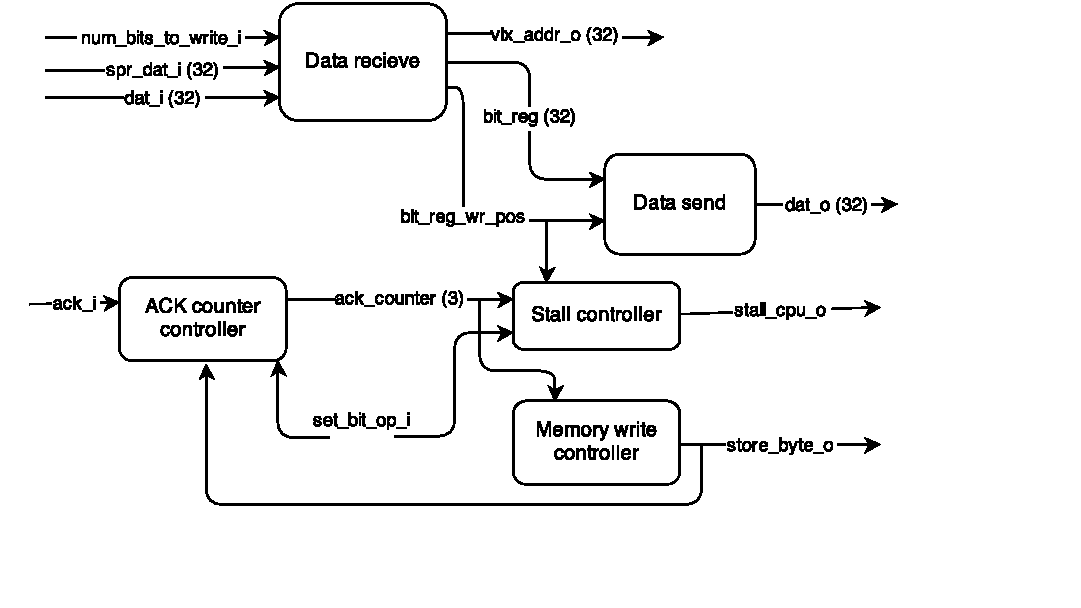
\includegraphics[width=1.0\textwidth]{blockschema.pdf}
\caption{Ett något förenklat blockschema för vår sbit-hårdvara.}
\label{fig:blockschema}
\end{figure}

\subsection{Data recieve}

Detta block ansvarar för att lägga in mottagen data i buffern, och
uppdatera pekaren för aktuell position. Adress- räknaren är även
inkluderad i detta block. Så här i efterhand hade det kanske varit mer
logiskt att placera den i ett separat block. Läsningen från data-bussen
sker i en enda klockcykel, genom att vår buffer bit\_reg skiftas åt
vänster för att göra plats för den nya datan, och OR:as med dat\_i.
Räknaren bit\_reg\_wr\_pos, som fungerar som en pekare till nästa lediga
element i buffern, räknas upp med så många bitar som just togs emot.\\

Eftersom att buffern skiftas åt vänster när den fylls på, befinner sig
data som nyss skickats någonstans i mitten av buffern. Detta göra att
denna modul även måste ha kod för att sätta de nyss skickade bitarna
till noll.\\


\subsection{Data send}

Denna modul lägger ut de bitar som skall skrivas
till minnet nästa gång i ett register som är kopplat till den utgående
databussen. Detta sker bara om det finns minst en byte i buffern, för
att undvika odefinierade signaler. Blocket ansvarar även för att
kontrollera om vi är på väg att skriva 0xFF till minnet, och alltså
måste skriva 0x00 till minnet härnäst.


\subsection{ACK counter}

Blocket sköter den ACK-räknare som räknas ner för varje ACK som tas
emot, och som alltså håller koll på det kvarvarande antalet ACK-signaler
som vi måste få från minnet innan vi är klara. Detta antal är givetvis
detsamma som det antal skrivningar vi måste göra. Vi skriver alltid en
byte åt gången, så fort vi fått ihop en hel byte, och får som mest två
nya bytes varje gång. Med andra ord behöver vi i normalfallet skriva en
eller två gånger, beroende på hur mycket data vi fått ihop i vår buffer.
För specialfallet med 0xFF krävs dock en extra skrivning av 0x00 direkt
efteråt, varför ACK-räknaren inte räknas ner i detta fall.


\subsection{Memory write}

Detta block hanterar styrsignalen för skrivning till minnet. Denna är
hög så länge ACK-räknaren indikerar att vi ännu inte skickat all data
till minnet, samt vi inte får någon ACK-signal. Write-signalen kommer
annars att bli en klockpuls för lång, vilket leder till att vi i så fall
skulle skriva två gånger till minnet istället för en gång.



\subsection{Stall controller}

Föga förvånande ansvarar detta block för att avgöra när en stall-signal
skall skickas. Vi tar det säkra före det osäkra och skickar alltid en
stall-signal samma klockpuls som set\_bit\_op\_i-signalen kommer,
oavsett om en skrivning till minnet behöver göras eller inte. Vi
fortsätter skicka stall-signal tills ACK-räknaren indikerar att vi inte
väntar på någon skrivning av data, d.v.s. efter en klockpuls om vi inte
behöver skriva något, eller klockpulsen efter att den sista ACK-signalen
från minnet har tagits emot, i annat fall.


\section{Resultat}

\subsection{Verifiering av hårdvarans funktion}

För att kontrollera att vår hårdvara fungerade, började vi med att
anropa vår instruktion från det montor-program som körs när datorn
startar. Efter en del felsökning och justering övergick vi till att
testa koden på en FPGA med samma monitor-program. Vi använde monitorns
inbyggda kommando för att visa minnesadresser för att verifiera att rätt
data skrevs till minnet. Ganska snabbt insåg vi behovet av att kunna
felsöka även i denna miljö utan att behöva syntetisera om koden varje
gång, och skrev därför testprogrammet asm.c som vi kunne ladda in i
minnet och köra via monitorn.\\

Det största problem vi hade under denna lab, och även det svåraste vi
fått under labkursen, var att sista biten i varje byte vi skrev till
minnet blev fel. Till skillnad från de tidigare fel vi fått under kursen
så fick vi varken några varningar av värde vid syntetiseringen, konstiga
odefinierade signaler eller märkliga läs/skrivcykler vid simulering.\\

Efter noggrannt studerande av syntesrapporten upptäckte vi att en
felaktig ihopslagning av två bitar i ett register orsakade problemet. Vi
gjorde om koden för skrivning till det aktuella registret. Simuleringen
blev fortfarande likadan som tidigare, men ingen konstig ihopslagning
gjordes vid syntetiseringen, vilket löste vårt problem.\\

Till sist testades även hårdvaran genom att instruktionen användes av
JPEG-acceleratorn. jchuff.c modifierades, för att använda set bit-
instruktionen för skrivning till minnet. Efter en rejäl stunds
felsökande genererades till sist en korrekt bild.\\


\subsection{Prestanda}

Vi använde vårt testprogram och den prestandaräknare som inkluderades i
jpegtest-programmet för att mäta prestandan på några olika slags anrop
till vår set bit-instruktion (Tabell \ref{tab:sbit_performance}). Dels
varierade vi storleken, dels testade vi även att enbart skriva 0xFF,
vilket i vår implementation gör två minnesskrivningar.\\

\begin{table}[ht]
    \centering
    \begin{tabular}{l l l}
        Storlek &  Data  &   Antal klockcykler\\
        \hline
        2       &  0x02  &   10\\
        8       &  0x33  &   13\\
        8       &  0xFF  &   17\\
        16      &  0x33  &   17\\
    \end{tabular}
    \caption{ Antal klockcykler per anrop av vår sbit-instruktion.
              Tabellen visar medelvärdet av 100 försök. }
    \label{tab:sbit_performance}
\end{table}

Vid användning i JPEG-acceleratorn jämförde vi utskriften av
prestandamätningen för en version av programmet som kompilerades utan
set bit-instruktionen (Tabell \ref{tab:jpeg_sw_performance}), mot
resultatet med denna instruktion påslagen (Tabell
\ref{tab:jpeg_sbit_performance}). Båda dessa versioner innehåller alla
de tidigare förbättringar som gjorts; hårdvaru-DCT samt DMA.

\begin{table}[ht]
    \centering
    \begin{tabular}{l l}
        Beskrivning & Antal klockcykler\\
        \hline
        Main program  & 25 847 242 \\
        Init  &  6 600 044 \\
        Encode\_image  & 19 247 198 \\
        Forward\_DCT  & 6 489 189 \\
        Copy  & 0 \\
        DCT kernel  & 0 \\
        Quantization  & 6 489 189 \\
        Huffman encoding  & 12 226 950 \\
        Emit\_bits  &  4 983 905 \\
    \end{tabular}
    \caption{ Prestanda för JPEG-acceleratorn utan sbit-instruktionen }
    \label{tab:jpeg_sw_performance}
\end{table}

\begin{table}[ht]
    \centering
    \begin{tabular}{l l}
        Beskrivning & Antal klockcykler\\
        \hline
        Main program  & 21 754 287 \\
        Init  & 6 653 818 \\
        Encode\_image  & 15 100 469 \\
        Forward\_DCT  & 6 396 157 \\
        Copy  & 0 \\
        DCT kernel  & 0 \\
        Quantization  & 6 396 157 \\
        Huffman encoding  & 8 126 873 \\
        Emit\_bits  & 1 306 129 \\
    \end{tabular}
    \caption{ Prestanda för JPEG-acceleratorn med sbit-instruktionen }
    \label{tab:jpeg_sbit_performance}
\end{table}

\subsection{FPGA-användning}
\begin{table}[ht]
    \centering
    \begin{tabular}{l l l}
        Flip Flops   &      7499 out of   46080  & 16\% \\
        4 input LUTs &      12519 out of  46080  & 28\% \\
        MULT18X18s   &      19 out of 120  &   15\% \\
        RAMB16s      &      42 out of 120  &   35\% \\
    \end{tabular}
    \caption{ De mest intressanta delarna ur syntes-rapporten för
              JPEG-acceleratorn med DCT, DMA samt sbit-instruktionen. }
    \label{tab:fpga_usage}
\end{table}

\section{Slutsats}

\subsection{Analys av prestanda}

Prestandan för set bit-instruktionen beror uteslutande på hur många
minnesaccesser som behöver göras vid anropet. Vid upprepade anrop med
storleken 2 görs en skrivning till minnet var fjärde anrop, vilket gör
att snitt-tiden blir lägre än i övriga fall. För storleken 8 görs en
skrivning vid varje anrop, vilket leder till värsta fallet på 13
klockcykler i medel. Vid skrivning av 0xFF görs internt två separata
skrivningar, vilket gör att detta tar exakt lika lång tid som
skrivningar av storleken 16, nämligen 17 cykler.\\

En intressant slutsats vi kan dra av detta är att det tar ganska mycket
overhead bara att utföra vår instruktion. För storlek 2 görs fyra gånger
färre minnesskrivningar jämfört med storlek 8, men tiden för dessa
skiljer sig bara med en tredjedel. På samma sätt görs dubbelt så många
skrivningar för storlek 16 som storlek 8 med samma data, men skillnaden
i exekveringstid dem emellan är mindre än en fjärdedel.\\

Instruktionen gjorde en hel del skillnad när vi använde den i JPEG-
acceleratorn. Som synes i Tabell \ref{tab:jpeg_sbit_performance}
minskade tiden för att skriva data till minnet vid Huffman-kodningen
(emit\_bits) från 5,0 miljoner cykler till 1,3 miljoner cykler. Den
totala tiden minskade därigenom med nästan lika mycket, vilket gav en
total prestandaökning med 16\%. Gruppen är dock enig om att
prestandaförbättring-per-timme-spenderad-i-Muxen-indexet troligen är
väldigt lågt.\\


\subsection{Möjliga förbättringar}

Ett problem med vår nuvarande hårdvara är att vi alltid skickar en
stall-signal till CPU:n så fort vi får in en set bit-instruktion. Detta
är i väldigt många fall inte alls nödvändigt (särskilt som vi bara
skriver till minnet om vi har en hel byte att skicka). Detta är särskilt
problematiskt i ett operativsystem med multitasking - det blir omöjligt
att göra saker parallelt om vi säger åt resten av datorn att sluta
arbeta så fort någon använder vår instruktion.\\

En möjlig förbättring skulle kunna vara att hårdvaran detekterar i vilka
fall som vi behöver skicka en stall-signal och inte. Detta behöver i så
fall ske med kombinatorik för att hinna skicka signalen tillräckligt
fort, i de fall där detta behövs. På så sätt skulle vi kunna lösa
problemen med dålig paralellism i operativsystem med multitaskning, samt
få något bättre prestanda generellt, på bekostnad av ganska lite
hårdvara.\\

Om målet istället skulle vara att hitta en billigare lösning på
bekostnad av prestanda, hade vi kunnat använda ett skiftregister för att
stegvis skifta in varje bit data i vårt register, istället för vår
nuvarande lösning som troligen realiseras med en stor samling
multiplexrar och OR-grindar för att lyckas göra detta på en
klockcykel.\\

\newpage
\begin{appendices}
\begin{changemargin}{-3cm}{-3cm}

\section{asm.c}
\lstinputlisting[language=C,caption={Testprogram för mätning av prestanda
                                     för sbit-instruktionen},label=asm]{asm.c}

\section{or1200\_vlx\_top.sv}
\lstinputlisting[language=Verilog,caption={Hårdvaruimplementationen för
                                           sbit-instruktionen},label=or1200_vlx_top]{or1200_vlx_top.sv}

\end{changemargin}
\end{appendices}

\end{document}
